\begin{enumerate}
	\item \textbf{Affirmation 1 : Fausse.}

	Calculons les coordonnées des vecteurs $\vectt{AB}$ et $\vectt{AC}$.

	Les coordonnées de $\vectt{AB}$ sont \quad $\begin{pmatrix}x_{\mathrm{B}} - x_{\mathrm{A}}\\ y_{\mathrm{B}} - y_{\mathrm{A}} \end{pmatrix} $
	\quad soit, avec les valeurs données : \quad $\begin{pmatrix} 3 - 2\\2-0 \end{pmatrix} $.

	Finalement :\quad $\vectt{AB} \begin{pmatrix} 1\\2 \end{pmatrix} $.

	De même, on a :\quad $\vectt{AC} \begin{pmatrix} 0 - 2\\4 - 0 \end{pmatrix} $,\quad soit \quad $\vectt{AC} \begin{pmatrix} -2\\4 \end{pmatrix} $.

	Comme le repère est orthonormé, on peut utiliser la formule analytique du produit scalaire :

	$\vectt{AB}\cdot\vectt{AC} = x_{\vectt{AB}}x_{\vectt{AC}} + y_{\vectt{AB}}y_{\vectt{AC}} = 1 \times (-2) + 2 \times 4 = -2 + 8 = 6.$

	Le produit scalaire n'est pas nul, donc les vecteurs $\vectt{AB}$ et $\vectt{AC}$ ne sont pas orthogonaux, et donc les droites (AB) et (AC), que ces vecteurs dirigent, ne sont pas perpendiculaires.

	\item Déterminons l'expression de la fonction dérivée $f'$. $f$ est un produit, et donc on applique la formule pour dériver un produit.

On peut poser :\quad $u : x \longmapsto 3x - 1$ \quad et $v$ la fonction exponentielle.

On a alors :\quad $u': x \longmapsto 3$\quad et $v'$ également la fonction exponentielle (celle-ci étant, par définition, égale à sa dérivée).

On a alors :\quad $f = uv$\quad et donc \quad $f' = u'v + uv'$.

On en déduit, pour tout $x$ réel :\quad $f'(x) = 3\e^{x} + (3x - 1)\e^{x} = (3 + 3x - 1)\e^{x} = (3x + 2)\e^{x}$.

\begin{enumerate}
\item \textbf{Affirmation 2. a. : Fausse.}

En effet, la fonction exponentielle est à valeurs strictement positives, donc $f'(x)$ est du signe de $(3x + 2)$, mais cette expression change de signe.

$\begin{aligned}
3x + 2 > 0 &\iff 3x > -2\\
			&\iff x > -\dfrac{2}{3} \quad \text{ car on divise par }3>0
\end{aligned}$

On a donc le tableau de signes pour $f'$:

\hfill~\begin{tikzpicture}
\tkzTabInit[lgt=3]{$x$/1, signe de $f'(x)$/1}{$-\infty$,$-\dfrac{2}{3}$,$+\infty$}
\tkzTabLine{,-,z,+,}
\end{tikzpicture}\hfill~

On peut en déduire que la fonction $f$ est strictement décroissante sur l'intervalle $\left]-\infty ; -\dfrac{2}{3}\right] $, ce qui contredit que la fonction serait croissante sur cet intervalle. Ainsi la fonction n'est pas croissante sur $\R$ tout entier.

\item \textbf{Affirmation 2. b. : Vraie.}

On applique la formule pour obtenir une équation de la tangente :\quad $y = f'(a) (x - a) + f(a)$.

Ici, la fonction $f$ est celle de l'énoncé, et l'abscisse $a$ est égale à 0.

On va donc calculer :\quad $f(0) = (3\times 0 - 1)\e^{0} = -1 \times 1 = -1$\quad et \quad $f'(0) = (3\times 0 + 2)\e^{0} = 2\times 1 = 2$.

Ainsi, une équation de la tangente cherchée est :\quad $y = 2 \times (x - 0) + (-1)$.

Une fois simplifiée, cette équation réduite est bien :\quad $y = 2x - 1$.
	\end{enumerate}
\end{enumerate}
